\section{Design and Implementation}
\label{sec.design}

\begin{figure*}
\centering
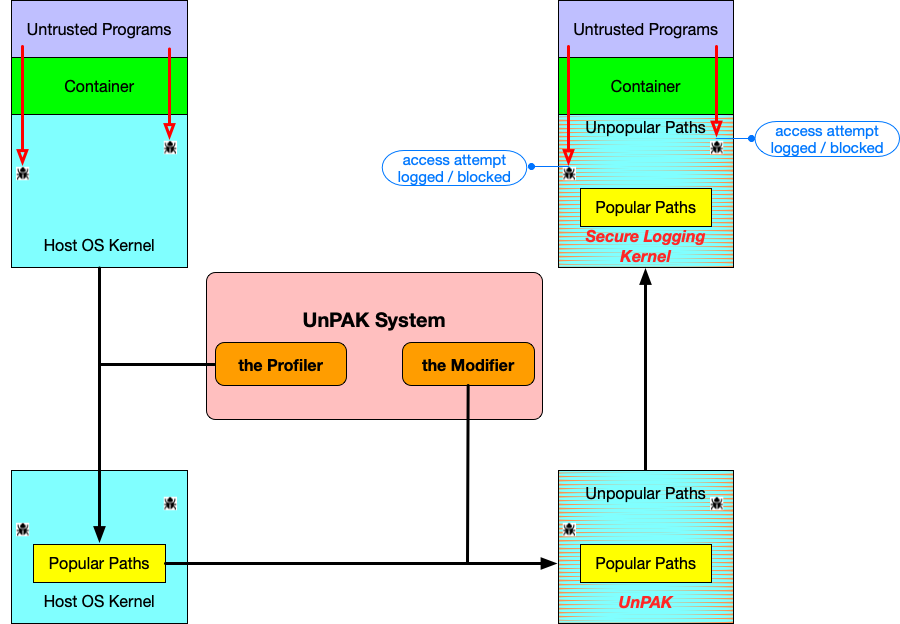
\includegraphics[width=2.0\columnwidth]{diagram/design.png}
\caption{\small Design overview of the UnPAK system}
\label{fig:design}
\end{figure*}

\begin{figure*}
\centering
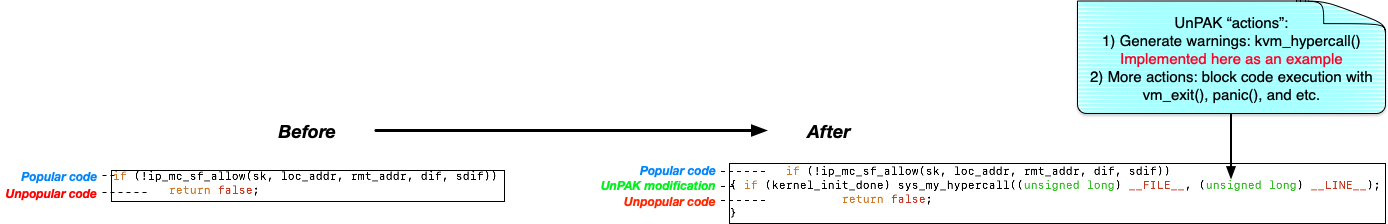
\includegraphics[width=2.2\columnwidth]{diagram/UnPAK-action.png}
\caption{\small Example of UnPAK actions}
\label{fig:UnPAKaction}
\end{figure*}

\begin{figure*}
\centering
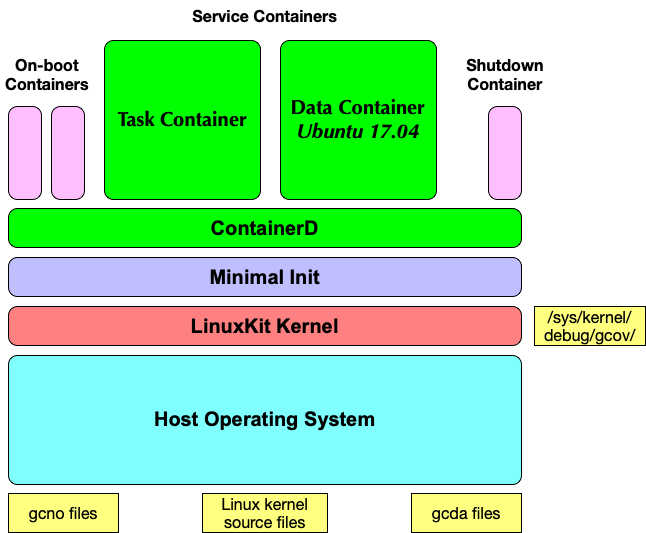
\includegraphics[width=1.5\columnwidth]{diagram/linuxkit-kernel-profiler.png}
\caption{\small Setting up Gcov profiler in LinuxKit}
\label{fig:linuxkit-kernel-profiler}
\end{figure*}

\subsection{Design}
\label{sec.design.design}

Designing an implementation of the popular paths metric for use with containers required completion of two separate tasks. 
First, we had to find the popular paths for the underlying host operating system. 
And, second, once we knew where these paths were, we needed a way to log / block the unpopular paths to warn and keep containers away from these less-used and potentially buggy code paths. Our solution was a dual module approach we call the \textbf{\textit{UnPopular Action Kernel (UnPAK) system}}, shown in Figure \ref{fig:design}. In this design, 
various security actions could be placed to guard the unpopular paths. In this work, we implemented a kernel logging system to provide security warnings as one instance of the 
potential actions to protect the system (shown in Figure \ref{fig:UnPAKaction}). 

Identifying the popular paths for a given container system is handled by the system module we refer to as the Profiler. 
The Profiler sets out a map highlighting places in the kernel that are safe for an application to access. 
It does so by identifying the lines of code executed  in the host kernel while running its default / regular workload, 
as defined in the configuration files (Dockerfiles) that come with the container images. We collected these lines of code, or the ``popular paths kernel traces,'' as we labeled them, 
from a set of the containers we ranked as “most popular” based on the number of user downloads. 

The second module, the Modifier, uses the map of safe access locations identified by the Profiler to find and adapt the rarely used paths to produce a tailored kernel, called the UnPAK. 
These risky paths are flagged to either generate security warning messages / logs, or to block code execution. 
(The process used to rework the kernel is described in more detail in the implementation section). 
The UnPAK can then be used to run containers without any required changes to the containers themselves.

\subsection{Implementation}
\label{sec.design.implementation}
This section describes in detail how the modules in our system were implemented.

\subsubsection{Implementing the Profiler}
\label{sec.implementation.profiler}
The Profiler is designed to collect the kernel trace of running user containers.
The kernel trace refers to the lines of code in the underlying host operating system kernel that were executed when running the regular container workload. 
The process used to obtain the kernel trace can be broken down into the following steps: 
\begin{enumerate}
	\item The Linux kernel used to run the Docker containers is recompiled with the Gcov \cite{gcov} kernel profiling feature enabled. 
	\item The Profiler automatically generates the configuration file for the Gcov-enabled LinuxKit. This file will define a task container running the main testing workload, along with a data container responsible for collecting, storing, and transferring the kernel trace data. (Shown in Figure \ref{fig:linuxkit-kernel-profiler}.) 
	\item The LinuxKit virtual machine is booted and a script in the profiler automatically starts running the workload of the task container. The profiler collects the kernel trace data, in the form of gcda files generated by Gcov, stores them at \texttt{/sys/kernel/debug/gcov/}, and, by the end of the run, transfers the data to the host system for further use. 
	\item The profiler uses the lcov \cite{lcov} tool to process the kernel trace data collected from the host system, and generates formatted data about which lines of code were executed in the kernel source files. This data will pinpoint which parts of the kernel are potentially risky and need to be marked. These sections will be instrumented by the Modifier to trigger an alert (or potentially another defensive action) if an application attempts to execute code in that path. 
\end{enumerate}

\subsubsection{Implementing the Modifier}
\label{sec.implementation.modifier}
The Modifier has three main parts: the Clang compiler, the Clang analyzer, and the kernel instrumenting tool (shown in Figure \ref{fig:linuxkit-kernel-modifier}). 
Its function is to identify the correct places in the source files to instrument, based on data extracted from the Profiler, and then to modify the code as needed. 

\begin{figure*}
\centering
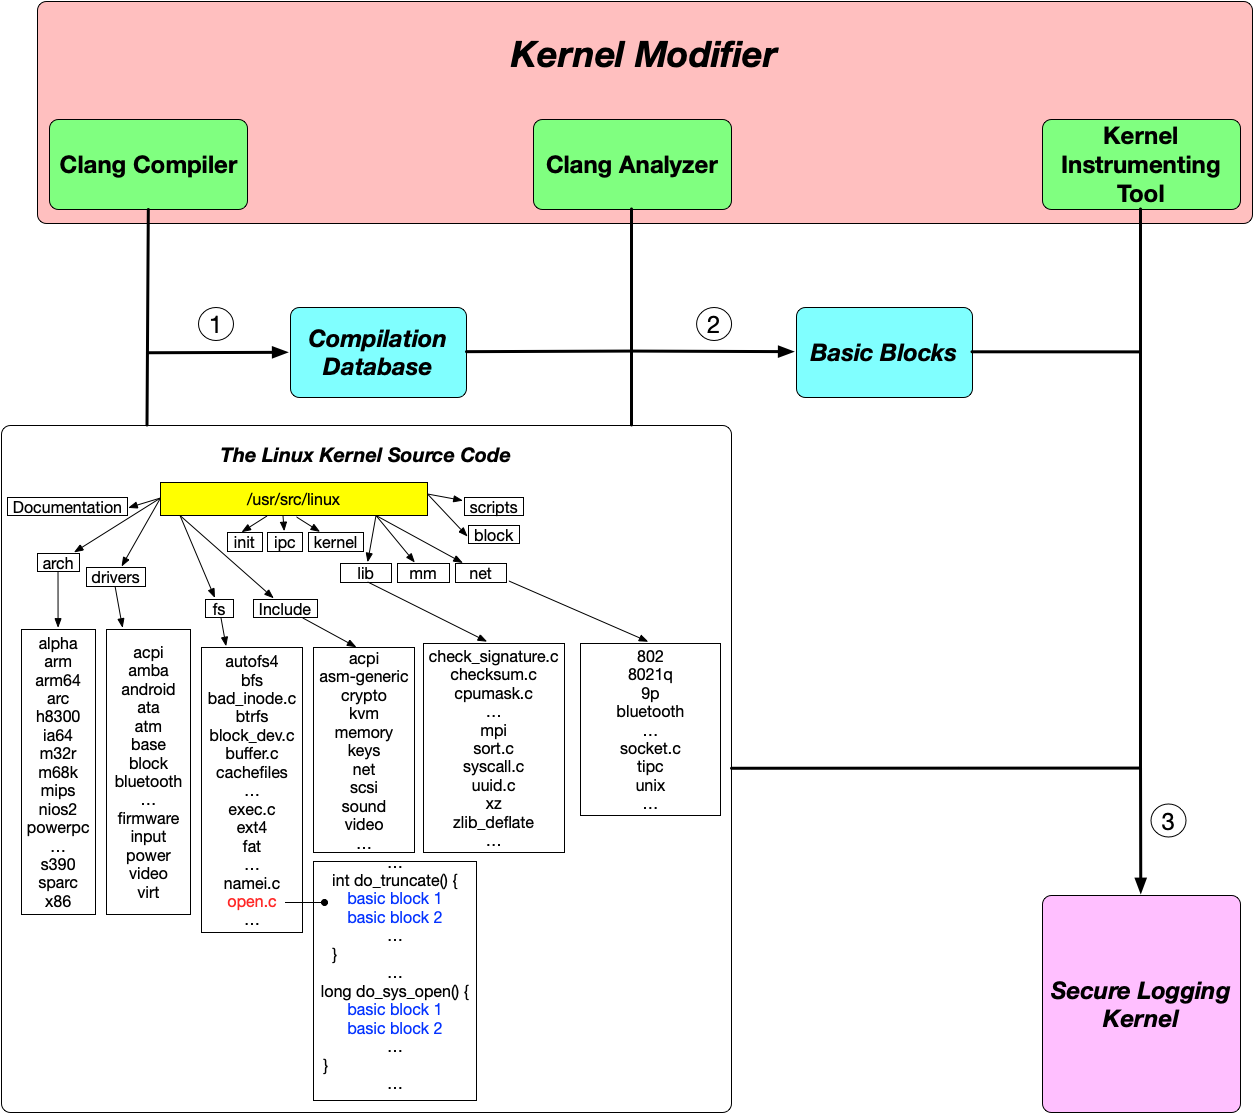
\includegraphics[width=1.5\columnwidth]{diagram/linuxkit-kernel-modifier.png}
\caption{\small Implementation of the Modifier}
\label{fig:linuxkit-kernel-modifier}
\end{figure*}

\begin{figure*}
\centering
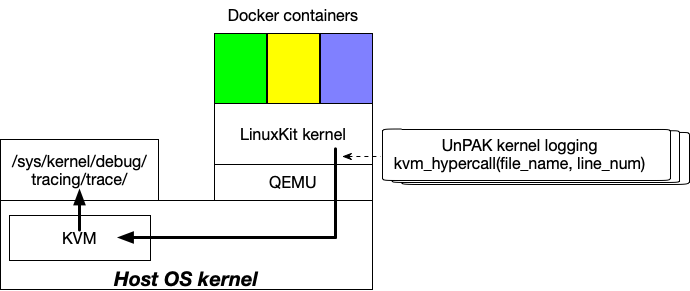
\includegraphics[width=1.5\columnwidth]{diagram/kvm_hypercall.png}
\caption{\small the KVM\_HYPERCALL implementation}
\label{fig:kvm_hypercall}
\end{figure*}

\begin{table}
%\begin{center}
\caption{Instrumentation code added to UnPAK}
\label{tab:kernel_instrumentation}
\begin{tabular}{c|c|c|c}
 kernel dir & unpopular & popular & total lines \\
 & functions & functions & inserted \\
 \hline
 arch & 1502 & 931 & 3325 \\
 \hline
 block & 774 & 245 & 1035 \\
 \hline
 crypto & 527 & 121 & 656 \\ 
 \hline
 drivers & 6290 & 2584 & 13305 \\
 \hline
 fs & 2108 & 1404 & 4883 \\
 \hline
 ipc & 198 & 42 & 249 \\
 \hline
 kernel & 3721 & 2120 & 6335 \\
 \hline
 mm & 1037 & 792 & 2954 \\
 \hline
 net & 4107 & 1746 & 7510 \\
 \hline
 security & 200 & 180 & 551 \\
 \hline
 \textbf{total} & \textbf{20464} & \textbf{10165} & \textbf{40803} \\
\end{tabular}
%\end{center}
\end{table}

The modifier operates in the following way: 
\begin{enumerate}
	\item The Clang C compiler from the Clang / LLVM project \cite{llvm}, along with a BEAR \cite{bear} tool compiles the Linux kernel source. Using BEAR, we can generate a compilation database containing all the compile flags and options needed for the process. In turn, this database will be used by our Clang analyzer to perform source code parsing in the next step.
	\item The Clang analyzer performs static analysis on the kernel source code to obtain the control flow graph for each function in the files. The analyzer leverages Clang's LibTooling \cite{clang-libtooling} to construct the AST tree from the kernel source code, and then obtain the control flow graph. With this graph, we can identify the corresponding source line number for each basic block. Furthermore, the beginning lines of all the blocks in the source files are candidates for places to add security logging code. Here, a \textbf{\textit{basic block}} refers to a straight-line code sequence with no branches in except to the entry and no branches out except at the exit. Thus, if a basic block is unpopular, it is sufficient to insert only one piece of secure logging code where it begins in order to alert users of any attempt to reach that code. This approach can optimize instrumentation by  avoiding redundancy in code injection. 
	\item The instrumenting tool executes modifications based on both the basic blocks, and the collected popular paths data. The algorithm for kernel modification directs the user through the basic blocks in the kernel source files. If none of the lines in a block are in the popular paths data, the block is considered unpopular , and the  instrumenting tool will add the security logging code,  a kvm hypercall from the LinuxKit kernel into the host Linux kernel (as shown in Figure \ref{fig:kvm_hypercall}) at the beginning. If we discover that an entire function has no lines in the popular paths data, we consider this an unpopular function, and just add our security logging code once where it starts. This allows us to avoid adding redundant and unnecessary code. These markers can guarantee minimal effect on the LinuxKit kernel functionality, while still being able to generate secure logging whenever unpopular paths are reached.  
	\item The Modifier automatically inserts secure logging code at the beginning of the unpopular paths in the Linux kernel source files and then recompiles the kernel to produce UnPAK. For non-popular functions that contained zero lines of popular code, we inserted one line of warning using the kvm hypercall at the beginning of each function. For popular functions, which have at least one line of popular code, we took the fine-grained approach to insert one line of warning code before each basic block that was unpopular. This tailored kernel can then be used to run Docker containers in the LinuxKit VM. 
\end{enumerate}

Table \ref{tab:kernel_instrumentation} presents an overview of the number of lines we inserted as security ``warnings'' in our kernel logging version implementation of UnPAK.  